%
%  -- INTRODUCCION --
%
\par Richard Lemarchand es un game designer prominente en la industria de videojuegos. Trabajó en franquicias populares, como Gex, Soul Reaver y Uncharted \cite{RichardLemarchandcom}. Además, es profesor en la Universidad de Southern California (USC) \cite{RichardLemarchandcom}. En 2021, publicó un libro llamado “A Playful Production Process” \cite{lemarchandPlayfulProductionProcess2021}, donde explora una metodología de desarrollo basada en su experiencia como game designer, productor y profesor. 
\par Para Lemarchand, hay una fuerte conexión entre game design y producción. Es por esto que en su metodología toma conceptos de ambos campos. De forma similar a Ramadan y Widyani, utiliza el libro "Game Design Workshop" \cite{fullertonGameDesignWorkshop2008} como punto de partida.
%
\begin{figure}[H]
  \centering
  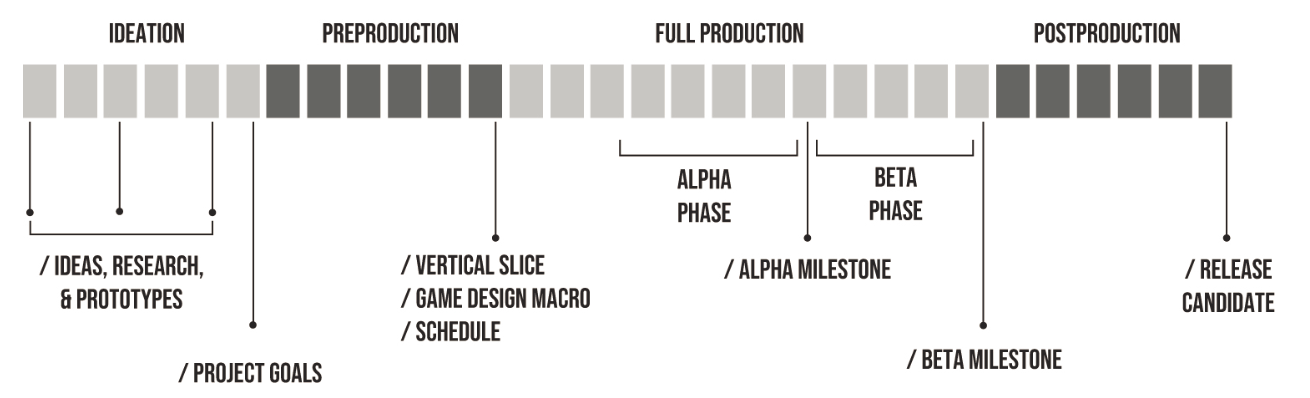
\includegraphics[width=\textwidth]{image6.png}
  \caption{Etapas de la metodología propuesta por Lemarchand. Extraída de \cite{lemarchandPlayfulProductionProcess2021}.}
  \label{fig:x proceso de desarrollo Lemarchand}
\end{figure}
%
%
%  -- IDEATION --
%
\subsection{Ideation}
\label{sec:ideation_lemarchand}
El proceso de desarrollo comienza en estae etapa, donde se definen una serie de objetivos llamados \textit{player experience goals}. Este concepto es propuesto por Fullerton, que los define como ``una serie de objetivos propuestos por el game designer, que indican el tipo de experiencia que los jugadores tendran durante el videojuego." \cite{fullertonGameDesignWorkshop2008} (Traducción propia).
\par Ejemplos de estos objetivos son ``los jugadores sentirán curiosidad por explorar un universo desconocido.'' o ``los jugadores colaborarán para sobrevivir un mundo post apocalíptico.''. Para establecer estos objetivos, Lemarchand propone una serie de herramientas:
\begin{itemize}
    \item Brainstorming: activadad grupal o individual donde se generan ideas espontáneamente. Lemarchand recomienda enfocarse en la cantidad de ideas, sin preocuparse por su calidad, resaltando la importancia de escribir todas las ideas, incluso las que parecen malas o irrelevantes.
    \item Mind mapping: esta técnica consiste en escribir una idea central y luego conectar ideas relacionadas. 
    \begin{figure}[H]
        \centering
        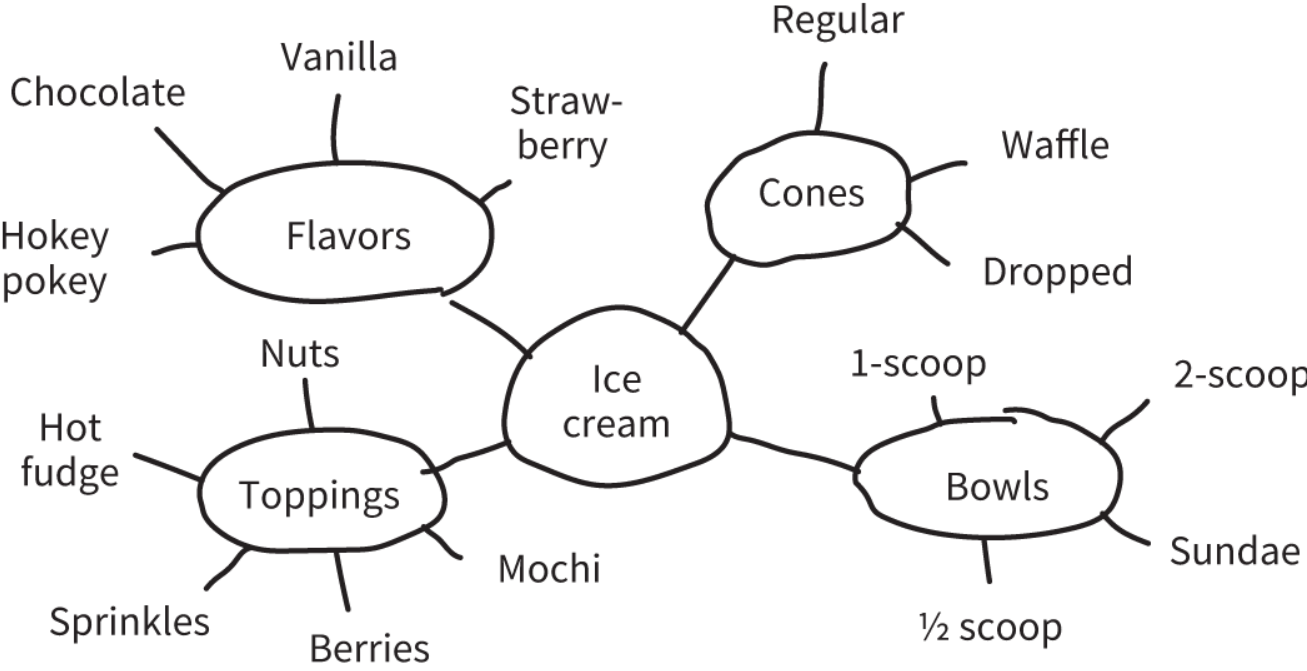
\includegraphics[scale=0.3]{mind_map.png}
        \caption{Ejemplo de un \textit{mind map}. Extraída de \cite{lemarchandPlayfulProductionProcess2021}.}
        \label{fig:x ejemplo de un mind map Lemarchand}
    \end{figure} 
    \item Automastim: este ejercicio consiste en configurar un temporizador y escribir sin parar durante un tiempo determinado. El objetivo es generar ideas espontaneamente, sin preocuparse por la calidad de las mismas.
\end{itemize}
%
%
\subsubsection{Prototipado}
\par Realizar prototipos es una parte fundamental de esta etapa. Lemarchand recomienda empezar con a prototipar lo antes posible, enfocandose en explorar distintas ideas. El objetivo de un prototipo es encontrar un número pequeño de mecánicas (inclusive una sola) que sea interesante o divertida. 
\par Para ayudar en la creación de prototipos, Lemarchand define algunos conceptos de game design. Primero define una \textit{mecánica} como ``reglas y procesos en un juego que lo vuelven funcional e interactivo.''(Traducción propia) \cite{lemarchandPlayfulProductionProcess2021}. Las mecánicas crean acciones llamadas \textit{game verbs}. Algunos ejemplos son saltar, caminar o disparar. Finalmente, define \textit{player activity} como ``el resultado de combinar mecánicas, \textit{game verbs} y narrativa con las acciones del jugador'' (Traducción propia) \cite{lemarchandPlayfulProductionProcess2021}. Por ejemplo, un jugador puede usar la barra espaciadora para ejecutar el \textit{game verb} de saltar. O puede ser un concepto mas abstracto, como tratar de encontrar un final diferente en una historia interactiva.
\par Estos conceptos son importantes porque para Lemarchand, un prototipo debe explorar un \textit{player activity} en particular para decidir si es interesante o no. Para ello, propone una serie de preguntas que un prototipo debe responder:
\begin{itemize}
    \item ¿Qué \textit{player activity} estoy prototipando?
    \item ¿Qué \textit{game verbs} estoy explorando?
    \item ¿Qué emocion evoca este \textit{player activity}?
    \item ¿Qué pregunta o idea se está evaluando con este prototipo?  
\end{itemize}
\bigbreak
\par Similar a Anderson, Lemarchand propone realizar tanto prototipos físicos como digitales. Los prototipos físicos son más rápidos de hacer, pero limitan el tipo de mecánicas que se pueden explorar. Por otro lado, los prototipos digitales son más lentos de hacer, pero permiten explorar una mayor variedad de mecánicas.
\par Playtesting es también una parte importante del proceso. Lemarchand recomienda entregar los prototipos a otras personas lo antes posible, y observar cómo interactuan con ellos. El objetivo es obtener feedback inmediato que informe las próximas iteraciones, notando lo que es interesante y divertido para los jugadores.
%
%
\subsubsection{Project goals}
\par El objetivo final de la etapa de \textit{Ideation} es definir los \textit{project goals}. La idea es que establecer objetivos claros para el proyecto ayuda a guiar el proceso de desarrollo en las siguientes etapas. Lemarchand separa los \textit{project goals} en dos categorias, \textit{experience goals} y \textit{design goals}. 
\bigbreak
\paragraph{Experience goal} Segun Lemarchand, un \textit{experience goal} es ``el tipo de experiencia que se le quiere dar al jugador, generalmente explicada en términos de la experiencia emocional.'' (Traducción propia) \cite{lemarchandPlayfulProductionProcess2021}. Ejemplos de esto puede ser la satisfacción de ganar o el miedo al jugar un juego de terror. La figura \ref{fig:x ejemplo de experience goals Lemarchand} muestra los \textit{experience goals} establecidos para Uncharted, uno de los juegos en los que trabajó el escritor.
%
\begin{figure}[H]
    \centering
    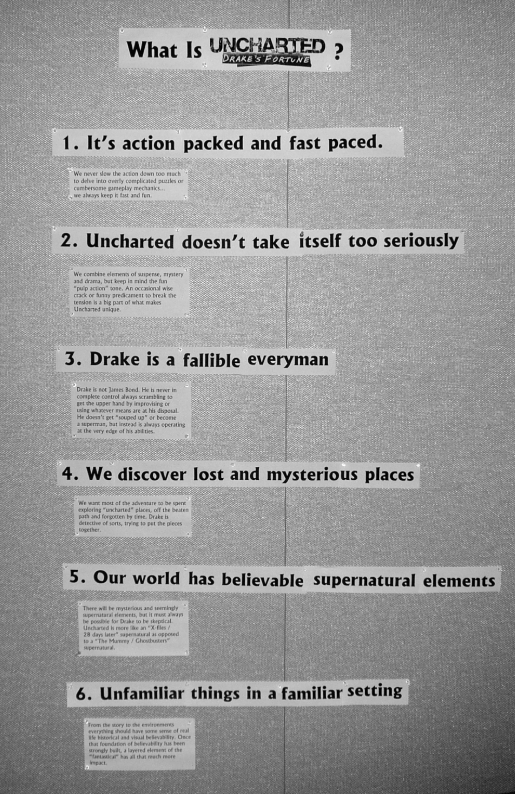
\includegraphics[scale=0.5]{experience_goals.png}
    \caption{``Experience goals'' del videojuego Uncharted. Extraída de \cite{lemarchandPlayfulProductionProcess2021}.}
    \label{fig:x ejemplo de experience goals Lemarchand}
\end{figure} 
%
\paragraph{Design goals} Por otro lado, los \textit{design goals} son las mecánicas que complementan a los \textit{experience goals}. Algunas categorias comunes son:
\begin{itemize}
    \item La plataforma en la que se desarrollará el videojuego (PC, consola, móvil, etc.).
    \item Mecánicas, \textit{game verbs} y \textit{player activities}.
    \item El género del videojuego (plataforma, aventura, rol, etc.).
    \item La dirección artística del videojuego (estilo visual, música, etc.).
\end{itemize}
\par Finalmente, Lemarchand remarca la importancia definir el público objetivo del juego. Para ello, recomienda añadir un \textit{project goal} indicando la audiencia, en el formato ``este juego está dirigido a [audiencia]''.
%
%
%  -- PRE PRODUCTION --
%
\subsection{Pre-production}
\par Lemarchand define a \textit{pre-production} (pre-producción en español) como la etapa donde se se establece el \textit{game design} y el plan a seguir durante la etapa de \textit{production}. Al final de esta etapa, se obtienen 3 artefactos: un \textit{vertical slice}, un \textit{game design macro} y un \textit{schedule}. 
%
%
\subsubsection{Vertical Slice}
Un \textit{vertical slice} es una demo de alta calidad de un videojuego \cite{lemarchandPlayfulProductionProcess2021}. Tanto gráficos, sonido, mecánicas y narrativa deben estar lo suficientemente pulidos como para ser considerados parte del producto final. 
\par Esta demo se construye iterativamente a partir de intentos anteriores, siguiendo un \hyperref[sec:modelos_evolutivos]{modelo evolutivo}. Para ello, se definen una  o varias mecánicas, se crea un prototipo para probarlas, se realiza \textit{playtesting} y se evalúa el resultado. Al final de cada iteración se revisa si el prototipo cumple con los \textit{experience goals} definidos, y si es necesario, se realizan cambios. Este proceso se repite hasta que se obtiene un \textit{vertical slice} que cumple con los objetivos del proyecto.
\begin{figure}[h]
    \centering
    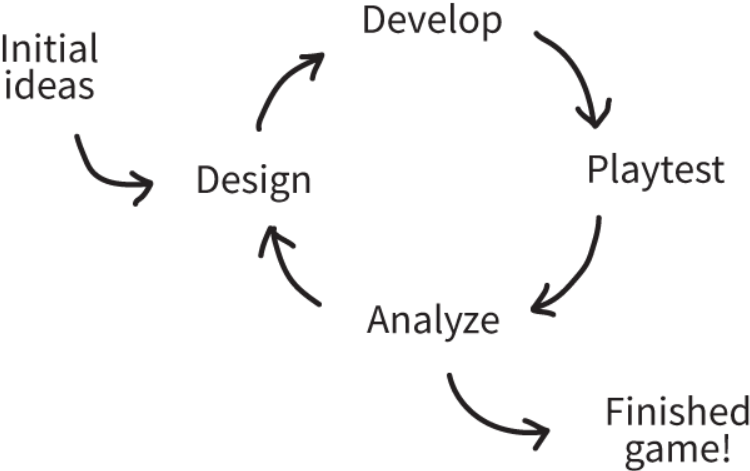
\includegraphics[scale=0.5]{vertical_slice_iteration.png}
    \caption{Proceso iterativo para la creación de un \textit{vertical slice}. Extraída de \cite{lemarchandPlayfulProductionProcess2021}.}
    \label{fig:x iteracion vertical slice}
\end{figure} 
\par Muchos juegos se construyen a partir de un patron repetitivo, llamado \textit{game loop}. Este patrón consiste en una serie de actividades que el jugador puede realizar, como atacar, disparar, saltar, etc. Luego, los \textit{game designers} crean distintas variaciones de estas actividades para mantener el interés del jugador. Este loop se debe ver representado en el \textit{vertical slice}, ya que es una parte fundamental del juego.
%
\par Durante el desarrollo del \textit{vertical slice} es escencial incorporar \textit{playtesting} como una parte fundamental del proceso. Este proceso debe realizarse tanto con otros miembros del equipo como con personas ajenas al proyecto. El objetivo es obtener feedback sobre el \textit{vertical slice} y evaluar si cumple con los \textit{experience goals} definidos. Para ello, Lemarchand propone una serie de prácticas:
\begin{itemize}
    \item \textbf{Minimizar la conversación con el jugador}: esto es útil para observar si el juego es intuitivo y entendible. 
    \item \textbf{Utilizar auriculares}: el sonido es una parte importante de la experiencia de juego, y puede guiar al jugador con el mismo.
    \item \textbf{Escribir los controles del juego en un papel}.
    \item \textbf{Escribir pistas para los problemas que ya se conocen}: es posible que la demo contenga algún bug  que requiera información adicional para que el jugador pueda continuar. En este caso, es recomendable escribir una pista para que el jugador pueda seguir jugando.
    \item \textbf{Sugerir que el jugador piense en voz alta}: el objetivo es obtener más información sobre la experiencia del jugador. Esto puede ayudar a identificar problemas que no son evidentes al observar al jugador.
    \item \textbf{Anotar las acciones del jugador}: escribir lo que el jugador va realizando en un papel puede ayudar a identificar tanto las partes interesantes del juego como las que generan problemas.
    \item \textbf{Realizar entrevistas luego de finalizar}: algunas preguntas recomendadas por Lemarchand son:
    \begin{itemize}
        \item ¿Cuál fue tu momento o interacción favorita?
        \item ¿Cuál fue tu momento o interacción que menos te gustó?
        \item ¿Hubo algo que quisieras hacer y que el juego no te permitiera? 
        \item Si pudieras cambiar algo del juego, ¿qué sería?
    \end{itemize}
\end{itemize}

\par Es importante analizar el feedback obtenido durante este proceso. Para ello, Lemarchand recomienda separar los datos en 3 categorías:
\begin{itemize}
    \item \textbf{Broken/must fix [roto/debe arreglarse]}: estos son problemas de \textit{game design} o bugs que impiden que el jugador tenga la experienca deseada, por lo que deben ser arreglados. Por lo general, la solución suele ser bastante obvia.
    \item \textbf{Question/maybe fix [pregunta/quizás deba arreglarse]}: estos son elementos que quizás no están funcionando correctamente, pero que requiere mayor investigación para determinar el por qué.
    \item \textbf{Suggestion/new idea [sugerencia/nueva idea]}: estas son sugerencias o ideas que pueden mejorar el juego, pero que no son necesarias para que el juego funcione correctamente. Por lo general, estas sugerencias se implementan en iteraciones posteriores.
\end{itemize}
%
%
\subsubsection{Concentric development}
\par Lemarchand propone utilizar \textit{concentric development} durante la etapa de pre-producción, el cual consiste en comenzar por el núcleo del juego y luego ir expandiendo con sistemas que lo complementan. De esta forma, el juego se construye en capas, donde para avanzar a la siguiente capa es necesario que la anterior esté lo suficientemente avanzada como para considerarse parte del producto final. En particular, Lemarchand propone 3 capas:
\begin{itemize}
    \item \textbf{Primary mechanics}: estas son las mecánicas fundamentales del juego. Por ejemplo, en un juego de plataformas, las mecánicas primarias se refiere al movimiento del personaje y de la cámara. A diferencia de la etapa de \textit{Ideation}, estas mecánicas deben ser lo suficientemente pulidas como para ser parte del producto final. Esto significa crear el arte, sonido y programacion y game design necesarios para considerarse completas.
    \item \textbf{Secondary mechanics}: estas mecánicas consisten en los \textit{game verbs} mas importantes del juego, generalmente aquellos que completan el \textit{game loop}. Por ejemplo, en un juego de plataformas, las mecánicas secundarias pueden saltar sobre enemigos o recoger objetos.
    \item \textbf{Tertiary mechanics}: estas mecánicas son las que complementan a las primarias y secundarias. Siguiendo el ejemplo del juego de plataformas, las mecánicas terciarias pueden ser las que permiten al jugador interactuar con el entorno, como abrir puertas o activar interruptores.
\end{itemize}
\par La ventaja de trabajar de esta forma es que al final de pre-producción, se obtiene un \textit{vertical slice} que contiene las mecánicas fundamentales del juego, y estas mecánicas estan lo suficientemente pulidas como para decidir si el proyecto debe continuar o no. 
%
%
\subsubsection{Game Design Macro}
\par Lemarchand define un \textit{game design macro} como ``una matriz de ideas que representa un overview del diseño del juego.'' (Traducción propia) \cite{lemarchandPlayfulProductionProcess2021}. Esta matriz enumera los aspectos más importantes del juego, sin enfocarse en los detalles. Por ejemplo, puede incluir el número de niveles o de personajes. Este artefacto es también una extensión de los \textit{project goals} definidos en la etapa de \textit{Ideation}. El \textit{game design macro} está compuesto de 2 partes: un documento llamado \textit{game design overview} y una tabla llamada \textit{macro chart}.
%
\paragraph{Game Design Overview} Este documento es una visión general del proyecto, y contiene una introducción a los elementos más importantes del juego, incluyendo mecánicas, narrativa y dirección artística. 
%
\paragraph{Macro Chart} Este documento fue originalmente ideado por el desarrollador Mark Cerny, quien lo describe como ``qué tipo de gameplay va en cada lugar'' (Traducción propia) \cite{academyofinteractivearts&sciencesDICESummit20022012}. La idea es que esta tabla contiene los niveles del juego, las mecánicas que se utilizan en cada uno, y los fragmentos de historia que suceden al jugar esa sección.
%
\begin{figure}[H]
    \centering
    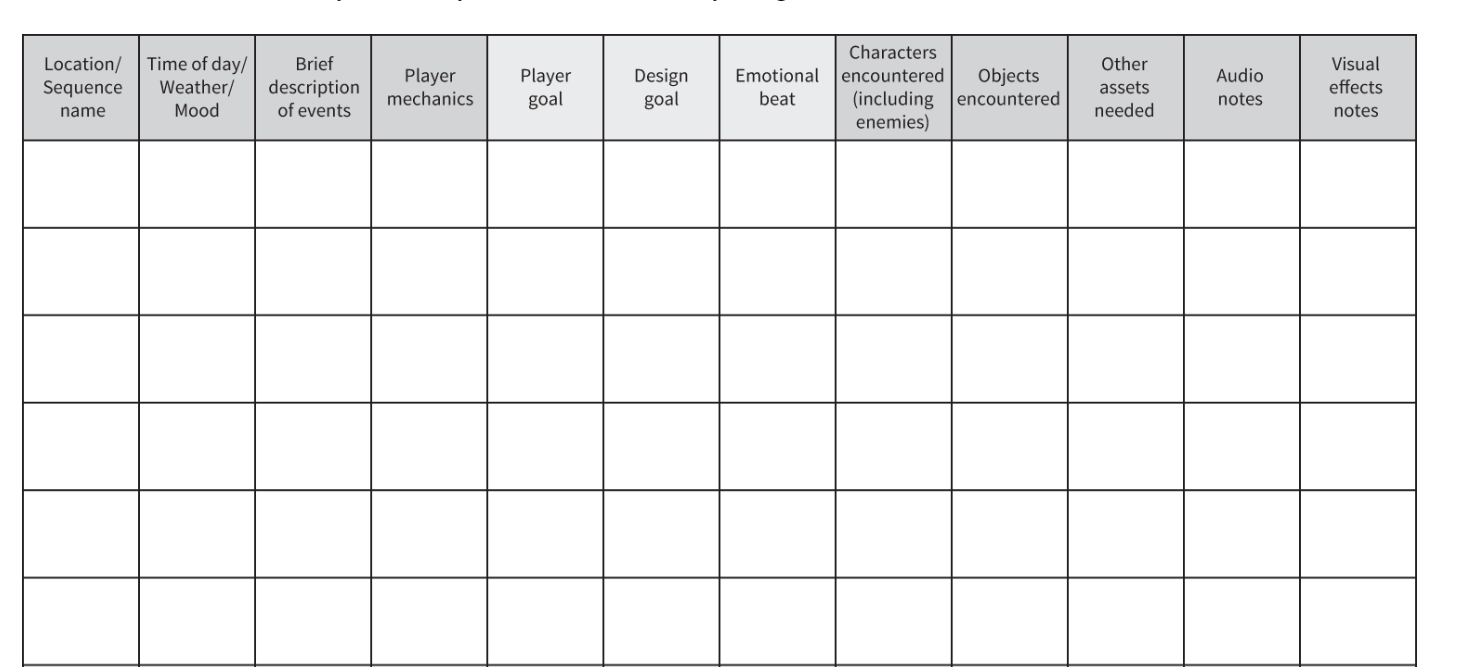
\includegraphics[width=\textwidth]{macro_chart.png}
    \caption{\textit{Macro chart} propuesto por Lemarchand. Extraída de \cite{lemarchandPlayfulProductionProcess2021}.}
    \label{fig:x macro chart}
\end{figure}
%
\par Las columnas \ref{fig:x macro chart} no son definitivas, sino que pueden variar dependiendo del proyecto. Sin embargo, Lemarchand pone énfasis en las siguientes:
\begin{itemize}
    \item \textbf{Player goal}: Lemarchand explica el concepto de \textit{autotelism}(``autolelismo'' en español). Este término, aplicado a videojuegos, se refiere a que cuando una persona juega un juego, establece objetivos para sí mismo basado en lo que el videojuego le permite hacer, lo que quieren hacer, lo que entienden que pueden hacer y lo que han experimentado de juegos similares \cite{lemarchandPlayfulProductionProcess2021}. En base a esta información, en la columna de \textit{player goal} se debe escribir el objetivo que el jugador debe cumplir en cada sección del juego. Un ejemplo de esto puede ser ``llegar al final del nivel'' o ``derrotar al jefe''.
    \item \textbf{Design goal}: a diferencia del \textit{player goal}, este objetivo está orientado a los \textit{game designers}, y consiste en lo que se desea lograr en términos de mecánicas y narrativa. Por ejemplo, ``introducir la mecánica de saltar'' o ``presentar un nuevo personaje''.
    \item \textbf{Emotional beat}: Esta columna describe lo que se desea que el jugador sienta al jugar esa sección del juego. Por ejemplo, ``sorpresa'' o ``alegría''.
\end 
{itemize}
\par Lemarchand llama \textit{sequences} (secuencias en español) a las filas de la tabla, donde cada una representa una sección del juego. Lemarchand propone una serie de conceptos que ayudan a definir su orden: 
\begin{itemize}
    \item \textbf{Secuenciar gameplay}: para Lemarchand, un buen punto de partida es considerar el orden en que se introducen las mecánicas del juego \cite{lemarchandPlayfulProductionProcess2021}. Por lo general, los \textit{game designers} crean secuencias que añaden mecánicas y dificultad progresivamente.
    \item \textbf{Secuenciar narrativa}: otra herramienta para definir el orden de las secciones es considerar la narrativa del juego. Por ejemplo, es necesario presentar a los personajes, el mundo en el que se desarrolla la historia, y los conflictos que deben resolver. Esto puede ayudar a definir el orden de las secciones del juego.
    \item \textbf{Secuenciar espacio}: otra forma de ordenar las secciones es considerar el espacio en el que suceden, especialmente si el juego está separado en niveles. Lemarchand destaca que crear espacios es una tarea que requiere mucho trabajo, por lo que es importante definir su orden y buscar maneras de reutilizar espacios.
\end{itemize}
\par Por otro lado, es importante considerar la duración de cada secuencia. Por ejemplo, para juegos grandes como \textit{Uncharted}, cada secuencia representa 15 minutos de juego. Para proyectos más pequeños cada sección puede durar entre 1 y 5 minutos. 
\par Finalmente, para completar el \textit{macro chart} se deben añadir el resto de pantallas importantes como el menú principal, el menú de pausa y opciones, y las pantallas de \textit{game over} \footnote{Pantalla que aparece cuando el jugador pierde en el juego.}, de carga y créditos.
%
%
\subsubsection{Schedule}
\par Durante pre-producción, el proceso de desarrollo es iterativo y no sigue un cronograma fijo. En cambio, para la etapa de producción es imperativo programar el progreso de desarrollo mediante un \textit{schedule} (cronograma en español).
\par Para comenzar este proceso, Lemarchand recomienda calcular lo que llama \textit{person-hour}. Este recurso consiste en la cantidad de horas que un miembro del equipo dedica al proyecto. El valor se calcula en base a la cantidad de semanas que se dedicarán al proceso de producción, el número de miembros del equipo y la cantidad de horas que cada uno dedica durante la semana.
\begin{equation}
    T = N \times P \times W
\end{equation}

donde:
\begin{itemize}
    \item $T$ = Total de \textit{person-hours} disponibles para el proyecto.
    \item $N$ = Número de miembros del equipo.
    \item $P$ = Horas-persona que cada miembro trabajará en una semana promedio.
    \item $W$ = Número de semanas dedicadas a producción.
\end{itemize}
\par Por ejmplo, para un equipo de 3 personas, que dedican 20 horas a la semana, durante 10 semanas, el total de \textit{person-hours} disponibles es:
\begin{equation}
    T = 3 \times 20 \times 10 = 600
\end{equation}
\par Luego, este número se compara con el número de \textit{person-hours} que se estima que se necesitan para completar todos los items del \textit{macro chart}, además de otras tareas como participar en reuniones o realizar \textit{playtests}.
\par Lemarchand recomienda comenzar con una tabla que contenga las tareas a realizar en conjunto con las siguientes columnas:
\begin{itemize}
    \item \textbf{Priority (prioridad)}: Esta columna indica la prioridad de cada tarea. Lemarchand propone 3 niveles:
    \begin{itemize}
        \item Priority 1 (prioridad 1): tareas obligatorias, que deben completarse para que el juego funcione correctamente. Por ejemplo, el movimiento del personaje, junto a sus animaciones, controles y sonidos.
        \item Priority 2 (prioridad 2): tareas que son importantes, pero que no son necesarias para que el juego funcione correctamente. Por ejemplo, los \textit{game verbs} utilizados por el jugador para interactuar con el mundo, como ``hablar'' o ``tirar objeto''.
        \item Priority 3 (prioridad 3): tareas que son opcionales, pero que pueden mejorar la experiencia del jugador. Por ejemplo, animaciones adicionales u objetos del entorno de juego.  
    \end{itemize}
    \item \textbf{Hours estimated (horas estimadas)}: Esta columna indica la cantidad de horas que se estima que se necesitan para completar cada tarea. Para Lemarchand, esta columna sólo puede tomar los valores de 1, 2, 4 u 8 horas. Aquellas tareas pequeñas se pueden agrupar en una sola, y las tareas que tomen más de 8 horas deben dividirse en subtareas más pequeñas. El objetivo es reducir la incertidumbre de las estimaciones, y que cada tarea sea lo suficientemente pequeña como para que se pueda estimar con precisión. 
    \item \textbf{Member assigned (miembro asignado)}: Esta columna indica el miembro del equipo que se encargará de cada tarea. Lemarchand recomienda asignar tareas a un solo miembro, ya que esto ayuda a evitar confusiones y conflictos.
\end{itemize} 
%
\begin{figure}[H]
    \centering
    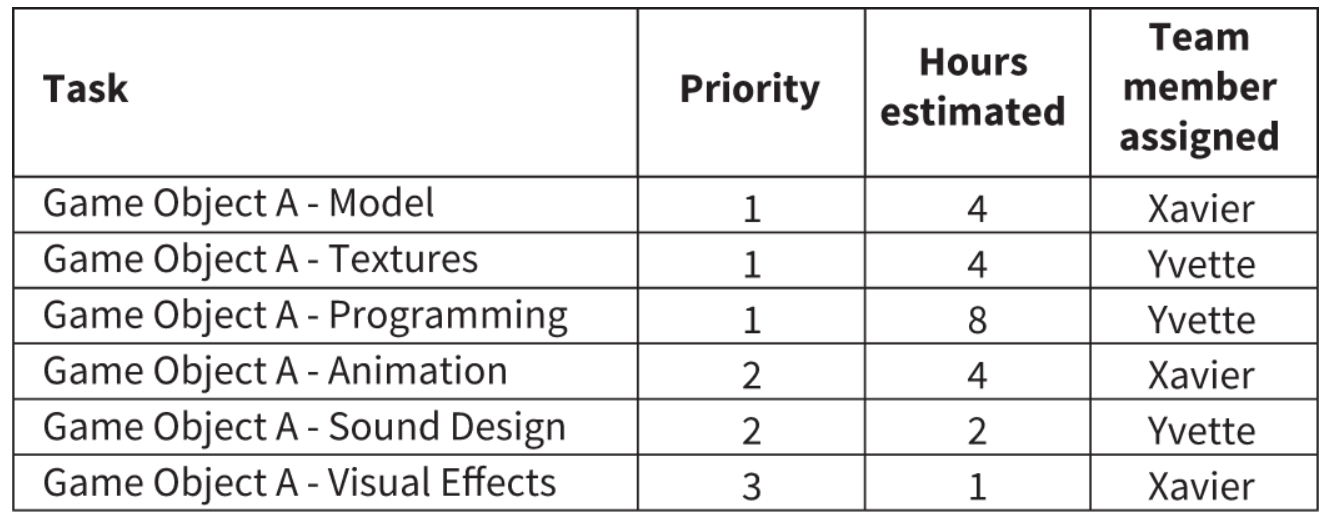
\includegraphics[width=\textwidth]{schedule_example.png}
    \caption{Ejemplo de un \textit{schedule}. Extraída de \cite{lemarchandPlayfulProductionProcess2021}.}
    \label{fig:x schedule ejemplo}
\end{figure}
%
\par Cabe destacar que esta comparación entre \textit{person-hours} disponibles y las horas estimadas para completar las tareas no es una estimación precisa, sino que es una forma de tener una idea general de si el proyecto es viable o no.
\bigbreak
\par Por otro lado, Lemarchand introduce 2 recursos de las metodologías ágiles: los \hyperref[sec:sprint]{sprints} y el \hyperref[sec:burndown_chart]{burndown chart}. Lemarchand separa el trabajo en \textit{sprints} de 2 semanas, y mide su avance mediante el \textit{burndown chart}, utilizando las horas de trabajo estimadas como indicador del progreso.
%
\begin{figure}[H]
    \centering
    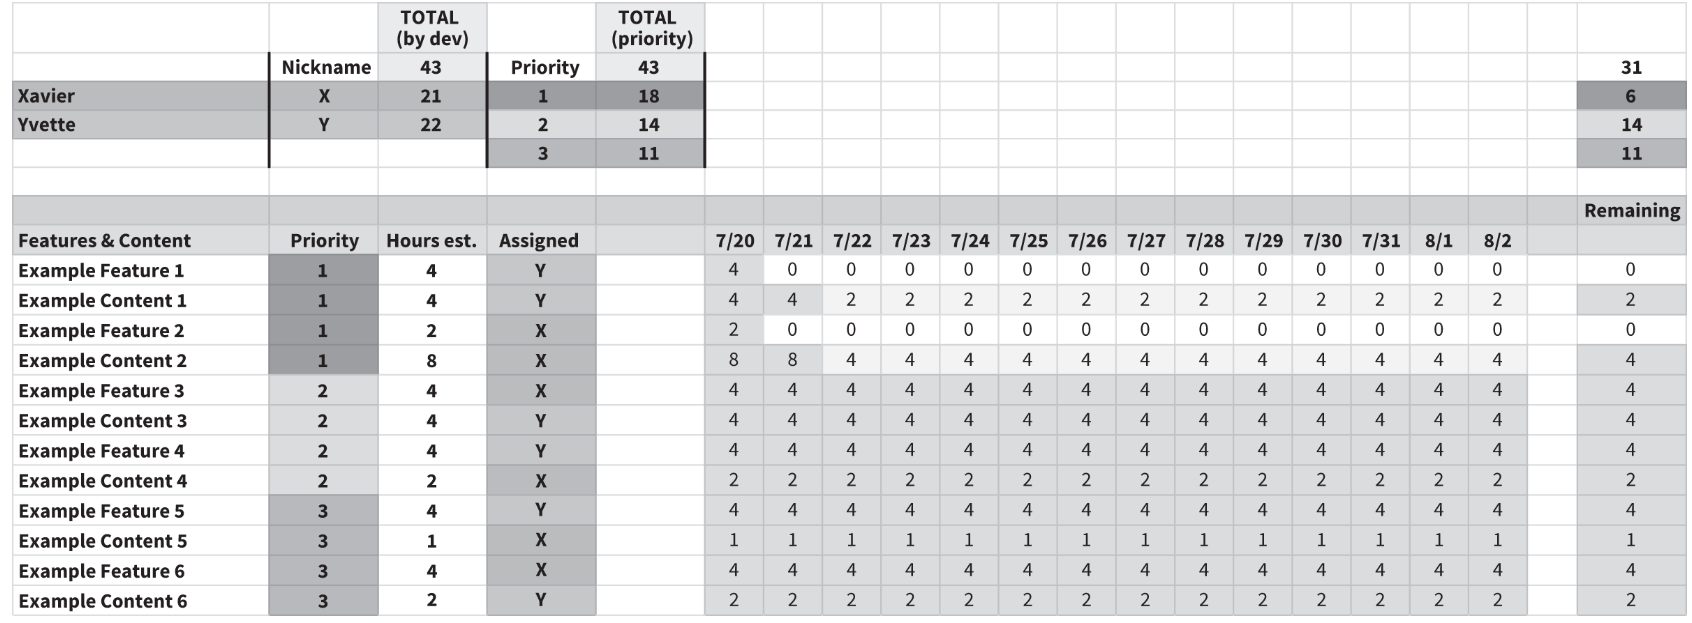
\includegraphics[width=\textwidth]{playful_production_burndown_chart.png}
    \caption{Ejemplo de un \textit{burndown chart} para un \textit{sprint} de 2 semanas. Extraída de \cite{lemarchandPlayfulProductionProcess2021}.}
    \label{fig:x burndown chart Lemarchand}
\end{figure}
%
\subsubsection{Milestone Review}
\par Al final de preproducción, Lemarchand recomienda realizar un \textit{milestone review}. En este evento, el equipo presenta el \textit{vertical slice} tanto a otros desarrolladores como \textit{stakeholders} y líderes del proyecto. El objetivo es obtener feedback sobre el progreso del proyecto y decidir si se debe continuar con la etapa de producción o no. Lemarchand propone una serie de etapas para realizar este evento:
\begin{enumerate}
    \item Los desarrolladores introducen el juego y explican el progreso del proyecto.
    \item Se realiza una demo del juego. Esta demo puede ser jugada por los desarrolladores o por un jugador externo.
    \item El grupo al que se presenta, ya sean \textit{stakeholders} u otros desarrolladores, realizan preguntas y comentarios sobre el juego.
\end{enumerate}
\par Luego de este evento, se debe decidir si el proyecto continúa a la etapa de producción. El proyecto puede no ser aprobado, pero con la posibilidad de realizar cambios y volver a presentar el \textit{vertical slice} en el futuro, o directamente cancelarse para trabajar en un juego distinto.
%
%
%  -- PRODUCTION --
%
\subsection{Production}
\par Si el \textit{vertical slice} es aprobado, el proyecto pasa a la etapa de \textit{production} (producción en español). En esta etapa, se implementan las mecánicas y sistemas definidos en el \textit{game design macro}, y se crea el contenido del juego. Esta etapa tiene 2 hitos principales:
\begin{itemize}
    \item \textbf{Alpha milestone}: en este punto se considera que el juego está en estado \textit{feature complete},es decir que todas las mecánicas y sistemas del juego están implementados, al menos de forma preliminar.
    \item \textbf{Beta milestone}: en este punto se considera que el juego está en estado \textit{content complete}, es decir que todo el contenido del juego está implementado, y sólo faltan ajustes finales y corrección de errores.
\end{itemize}
\par En esta sección se profundiza sobre estos hitos, además de las herramientas que Lemarchand propone para esta etapa.
%
%
\subsubsection{Formal playtesting}
\par Antes de expandir sobre las fases de \textit{Alpha} y \textit{Beta}, Lemarchand introduce el concepto de \textit{formal playtesting}. Comenzando cerca del final de la fase de \textit{Alpha}, Lemarchand propone realizar eventos regulares de \textit{playtesting}, donde se busca obtener datos rigurosos sobre la experiencia del jugador. Este evento se diferencia del \textit{playtesting} informal que se realiza durante la etapa de \textit{Pre-production}, introduciendo una nueva serie de prácticas y herramientas:
\paragraph{Formal Playtest Survey} Se introduce una encuesta que se le entrega al jugador luego de jugar el videojuego. Esta encuesta contiene preguntas sobre la experiencia del jugador, y permite obtener datos cuantitativos y cualitativos sobre el juego. Lemarchand recomienda estructurar las preguntas utilizando la escala Likert, en la cual la respuesta se presenta en una escala gradual, generalmente de 1 a 5, donde 1 representa la respuesta más negativa y 5 la más positiva. La figura \ref{fig:x escala Likert Lemarchand} muestra un ejemplo de este tipo de pregunta, en particular cuestionando si el jugador disfrutó de la calidad de los gráficos del juego.
\begin{figure}[H]
    \centering
    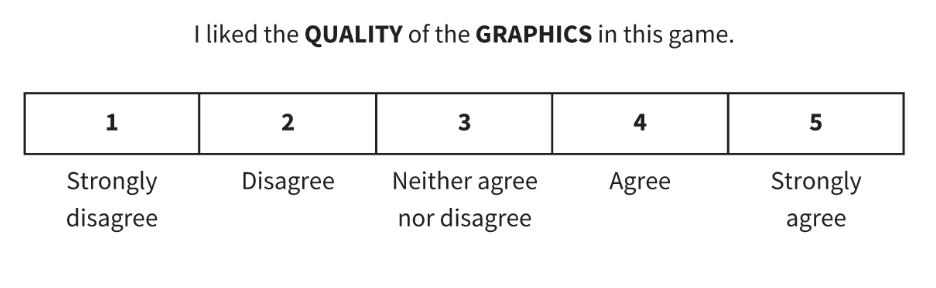
\includegraphics[width=\textwidth]{likert_scale_example.png}
    \caption{Ejemplo de un una pregunta en formato de escala Likert. Extraída de \cite{lemarchandPlayfulProductionProcess2021}.}
    \label{fig:x escala Likert Lemarchand}
\end{figure}
\paragraph{Exit interview} Luego de la encuesta, Lemarchand recomienda realizar una entrevista al jugador, esta vez con preguntas abiertas. Algunas preguntas recomendadas son:
\begin{itemize}
    \item ?`Cómo te hizo sentir x parte del juego?
    \item Describe cómo realizar x acción en el juego.
    \item Describe cómo x sistema funciona. (ej: sistema de inventario)
    \item Describe x personaje. ?`Quién es? ?`Cómo te hizo sentir?
    \item Describe una parte del juego donde te hayas sentido perdido.
\end{itemize}
\paragraph{Game Metrics} Otra herramienta propuesta por Lemarchand es recopilar datos del juego mientras los jugadores realizan el \textit{playtest}. Estos datos pueden incluir el tiempo que el jugador pasa en cada sección del juego así como las distintas acciones que realizan. Esta información pueden ayudar a identificar problemas de diseño y mejorar la experiencia del jugador. Por ejemplo, Lemarchand menciona cómo arreglaron un problema de diseño donde el jugador trataba de utilizar un sistema que permite escalar ciertas estructuras en las zonas incorrectas. Para ello, almacenaron los lugares donde los jugadores saltaban y luego observaban si estos lugares eran los correctos o no.
\begin{figure}[H]
    \centering
    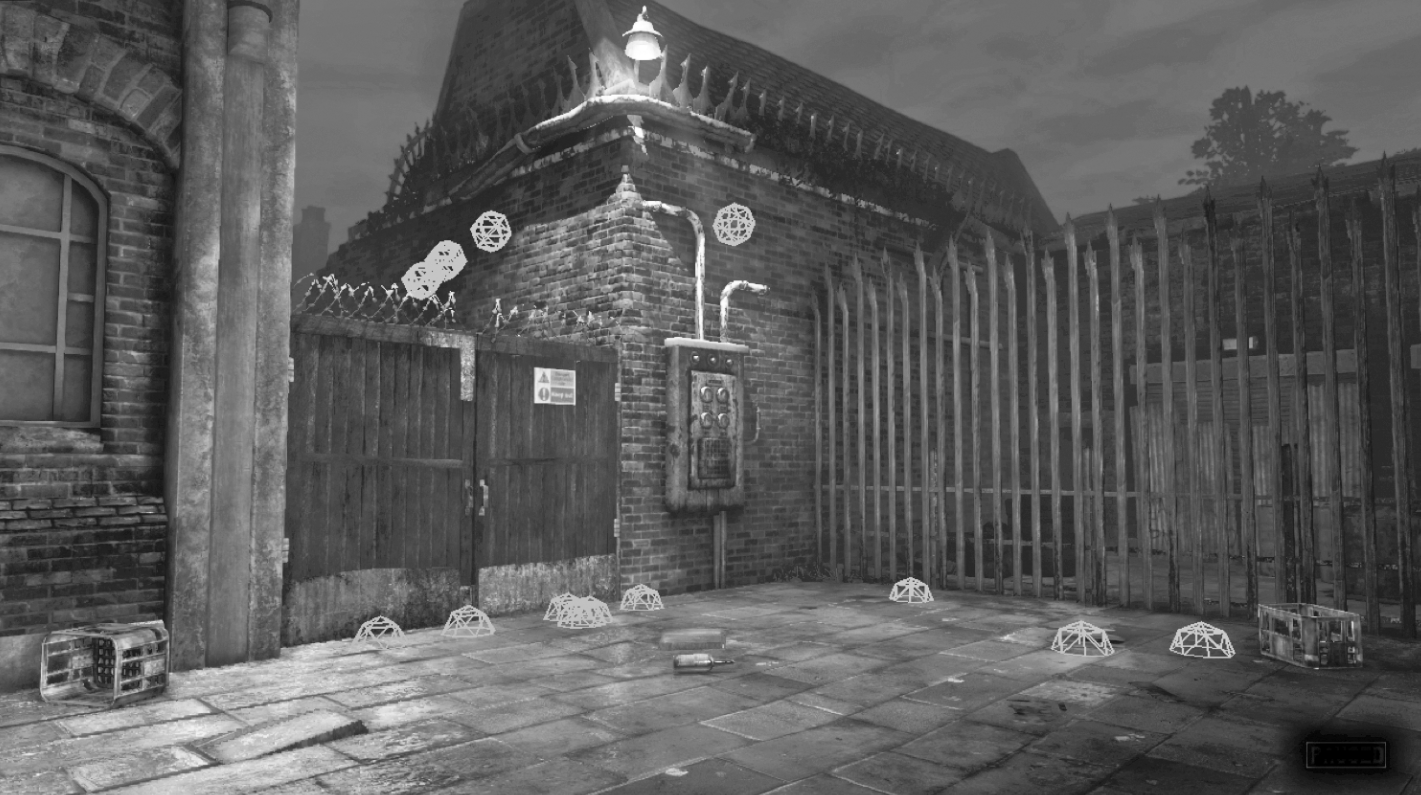
\includegraphics[width=\textwidth]{jump_metrics_example.png}
    \caption{Ejemplo de métricas en el juego \textit{Uncharted}. Las circunferencias indican los lugares donde el jugador realizó saltos. Extraída de \cite{lemarchandPlayfulProductionProcess2021}.}
    \label{fig:x metricas de salto Uncharted Lemarchand}
\end{figure}
%
%
\subsubsection{Alpha Phase}
\par Durante esta fase, los desarrolladores trabajan en completar las mecánicas y sistemas del juego. El objetivo es llegar al \textit{alpha milestone}, donde se considera que el juego esta en estado \textit{feature complete} y \textit{sequence complete}.
\par Lemarchand define una \textit{feature} (funcionalidad en español) como una pieza de funcionalidad dentro del juego \cite{lemarchandPlayfulProductionProcess2021}. Por ejemplo, en un juego de plataformas, una \textit{feature} puede ser el sistema de salto del personaje. Por otro lado, define un \textit{content} (contenido en español) como los \textit{assets} que componene el juego, ya sean sonidos, modelos 3D, texturas, etc. \cite{lemarchandPlayfulProductionProcess2021}. Siguiendo el caso de un juego de plataformas, el contenido puede ser el modelo del personaje, los enemigos y los escenarios. Así, se describen los estados anteriormente mencionados:
\begin{itemize}
    \item \textbf{Feature complete}: Un juego se considera \textit{feature complete} cuando todas las mecánicas y sistemas del juego están implementados, al menos de forma preliminar. Lemarchand recomienda que al menos haya una de cada mecánica en el juego. Por ejemplo, si en el producto final habrá un sistema para hablar con personajes, en la fase de \textit{Alpha} debe haber al menos un personaje y una conversación con el mismo. No es necesario que estén todos los personajes o conversaciones, pero si al menos uno de cada tipo.
    \item \textbf{Sequence Complete} El juego está en estado \textit{sequence complete} cuando todos los niveles están implenentados en el juego, al menos de forma preliminar. El objetivo es que sea posible jugar de principio a fin de forma que se pueda evaluar el ritmo del proyecto \cite{lemarchandPlayfulProductionProcess2021}. Para lograr este estado también se deben implementar los menús como menú principal, de pausa o pantalla de carga.
\end{itemize}
\par Por otro lado, Lemarchand propone diseñar el comienzo del juego en esta etapa. Esta parte del videojuego es muy importante porque es la primera impresión que el jugador tiene del mismo, por lo que debe ser lo suficientemente llamativa e interesante para que quiera seguir jugando. En esta primera parte del juego se deben introducir los controles y las mecánicas principales, además de un gancho narrativo que los mantenga interesados.
\par Además, en esta etapa se comienza el proceso de marketing del producto. Similar a Anderson, Lemarchand recomienda un \textit{press kit} con información sobre el juego, como imagenes y videos, además datos sobre el equipo de desarrollo y el proyecto. Además, recomienda comenzar a publicitar el juego en redes sociales, si embargo no indica herramientas para llevarlo a cabo. Por otro lado, coincide con Anderson en la importancia de contactar con creadores de contenido que tengan una audiencia similar a la del proyecto.
\par Finalmente, durante esta etapa es recomendable implementar un sistema de \textit{bug tracking} (seguimiento de errores en español) que permita registrar errores dentro del juego. En particular, es importante observar:
\begin{itemize}
    \item Errores en los sistemas de juego, como mecánicas que no funcionan correctamente o que no son intuitivas.
    \item Errores en el contenido del juego, como modelos 3D que no se ven bien o texturas que no se cargan correctamente.
    \item Performance del juego, como caídas de frames o tiempos de carga largos.
    \item Problemas de game design, como mecánicas que no son divertidas o que no cumplen con los \textit{experience goals} definidos.
\end{itemize}
\bigbreak
\par Esta etapa concluye con el \textit{alpha milestone}, donde se presenta el progreso del juego tanto a personas ajenas al proyecto como al equipo de desarrollo. El equipo debe presentar la audiencia objetivo, el estado del proyecto (si pueden avanzar a la siguiente etapa o no) y los problemas conocidos del proyecto. En base a esta información, se continúa a la siguiente etapa, la fase de \textit{beta}.
%
%
\subsubsection{Beta Phase}
\par En esta fase se busca llegar al estado \textit{content complete}. Para ello, todas las mecánicas y contenido del juego deben estar implementados lo suficientemente pulido como para ser parte del producto final. Esto incluye:
\begin{itemize}
    \item Todas las mecánicas y sistemas del juego.
    \item Todo el contenido del juego.
    \item Todos los niveles, jugables de principio a fin.
    \item Todos los menús, incluyendo el menú principal, de pausa y de opciones.
    \item El arte para tiendas digitales, incluyendo iconos y material promocional.
\end{itemize}
\par Lemarchand también recomienda accionar sobre los errores de sistemas o diseño que se comenzaron a anotar durante la etapa de \textit{alpha}. No es necesario arreglar todos los errores, pero si aquellos que son más importantes o que afectan la experiencia del jugador.
\bigbreak
\par Esta etapa finaliza en el \textit{beta milestone}. De forma similar al \textit{alpha milestone}, el equipo presenta el progreso del proyecto con el objetivo es obtener feedback sobre el juego y formar un plan con el que continuar a la siguiente etapa. Además, Lemarchand recomienda realizar reuniones internas para discutir las tareas a realizar durante la siguiente fase, \textit{post production} (o post producción en español). 
%
%
%  -- PRODUCTION --
%
\subsection{Post Production}
\par Esta etapa es la última del proceso de desarrollo, y se centra en 3 actividades: \textit{bug fixing} (arreglo de errores), \textit{polishing} (pulido) y \textit{balancing} (balance de diseño). El objetivo es preparar el juego para su lanzamiento, y asegurar que esté en un estado óptimo para los jugadores.
\begin{itemize}
    \item \textbf{Bug fixing}: durante esta etapa se pone un fuerte énfasis en arreglar los errores que se hayan encontrado durante el proceso de producción. El resto de tareas se detienen en favor de esta, y cada cambio se prueba exhaustivamente para asegurarse de que no se introduzcan nuevos errores.
    \item \textbf{Polishing}: esto consiste en realizar pequeños cambios que mejoren la experiencia del jugador. Estos cambios no deben ser grandes, ya que pueden introducir nuevos errores.
    \item \textbf{Balancing}: esta actividad consiste en ajustar las mecánicas del juego para que sean justas y divertidas. Similar al proceso de \textit{polishing}, se recomienda realizar cambios pequeños para evitar nuevos \textit{bugs}.
\end{itemize}
\par En base a estos cambios, se crea un artefacto llamado \textit{release candidate}, el cual se refiere a una \textit{build} del juego que se cree que está lista para ser lanzada. Para ello, el proyecto es tanto \textit{feature complete} como \textit{content complete}, y se han arreglado todos los errores conocidos, además de pasar por un proceso de \textit{polishing} y \textit{balancing}.
\par Finalmente, se realiza un proceso exhaustivo de pruebas para asegurarse que no se encuentra ningun otro error. Si no se encuentran problemas, se obtiene el artefacto \textit{gold master}, el cual es la versión final del juego. 


